\begin{figure}
  \centering
  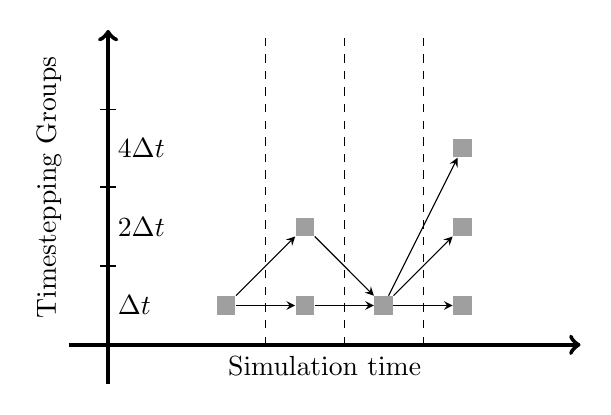
\begin{tikzpicture}
    \draw[->,ultra thick] (-1,-0.5)--(-1,4);
    \node[rotate=90] at (-1.75, 2)  (a) {Timestepping Groups};
\draw[->,ultra thick] (-1.5,0)--(5,0) node[midway,below]{Simulation time};

    \draw[|-|] (-1,0)--(-1,1) node[midway,right] {$\Delta t$};
    \draw[|-|] (-1,1)--(-1,2) node[midway,right] {$2 \Delta t$};
    \draw[|-|] (-1,2)--(-1,3) node[midway,right] {$4 \Delta t$};

\draw[dashed] (1,0)--(1,4);
\draw[dashed] (2,0)--(2,4);
\draw[dashed] (3,0)--(3,4);

\begin{scope}
    \node[fill=darkgray!50] (AI) at (0.5,0.5) {};
    \node[fill=darkgray!50] (AII) at (1.5,0.5) {};
    \node[fill=darkgray!50] (AIII) at (2.5,0.5) {};
    \node[fill=darkgray!50] (AIV) at (3.5,0.5) {};
    \node[fill=darkgray!50] (BI) at (1.5,1.5) {};
    \node[fill=darkgray!50] (BII) at (3.5,1.5) {};
    \node[fill=darkgray!50] (CI) at (3.5,2.5) {};
\end{scope}

\begin{scope}[>=stealth,black]
  \path[->] (AI) edge (AII);
  \path[->] (AI) edge (BI);
  \path[->] (AII) edge (AIII);
  \path[->] (BI) edge (AIII);
  \path[->] (AIII) edge (AIV);
  \path[->] (AIII) edge (BII);
  \path[->] (AIII) edge (CI);
\end{scope}

  \end{tikzpicture}
\caption{Illustration of conservative parallel discrete event simulation with no look ahead.}
\label{fig:cons}
\end{figure}